% --> Packet transactions and how this is different from other transactions.
\section{Packet transactions}
\begin{figure}
  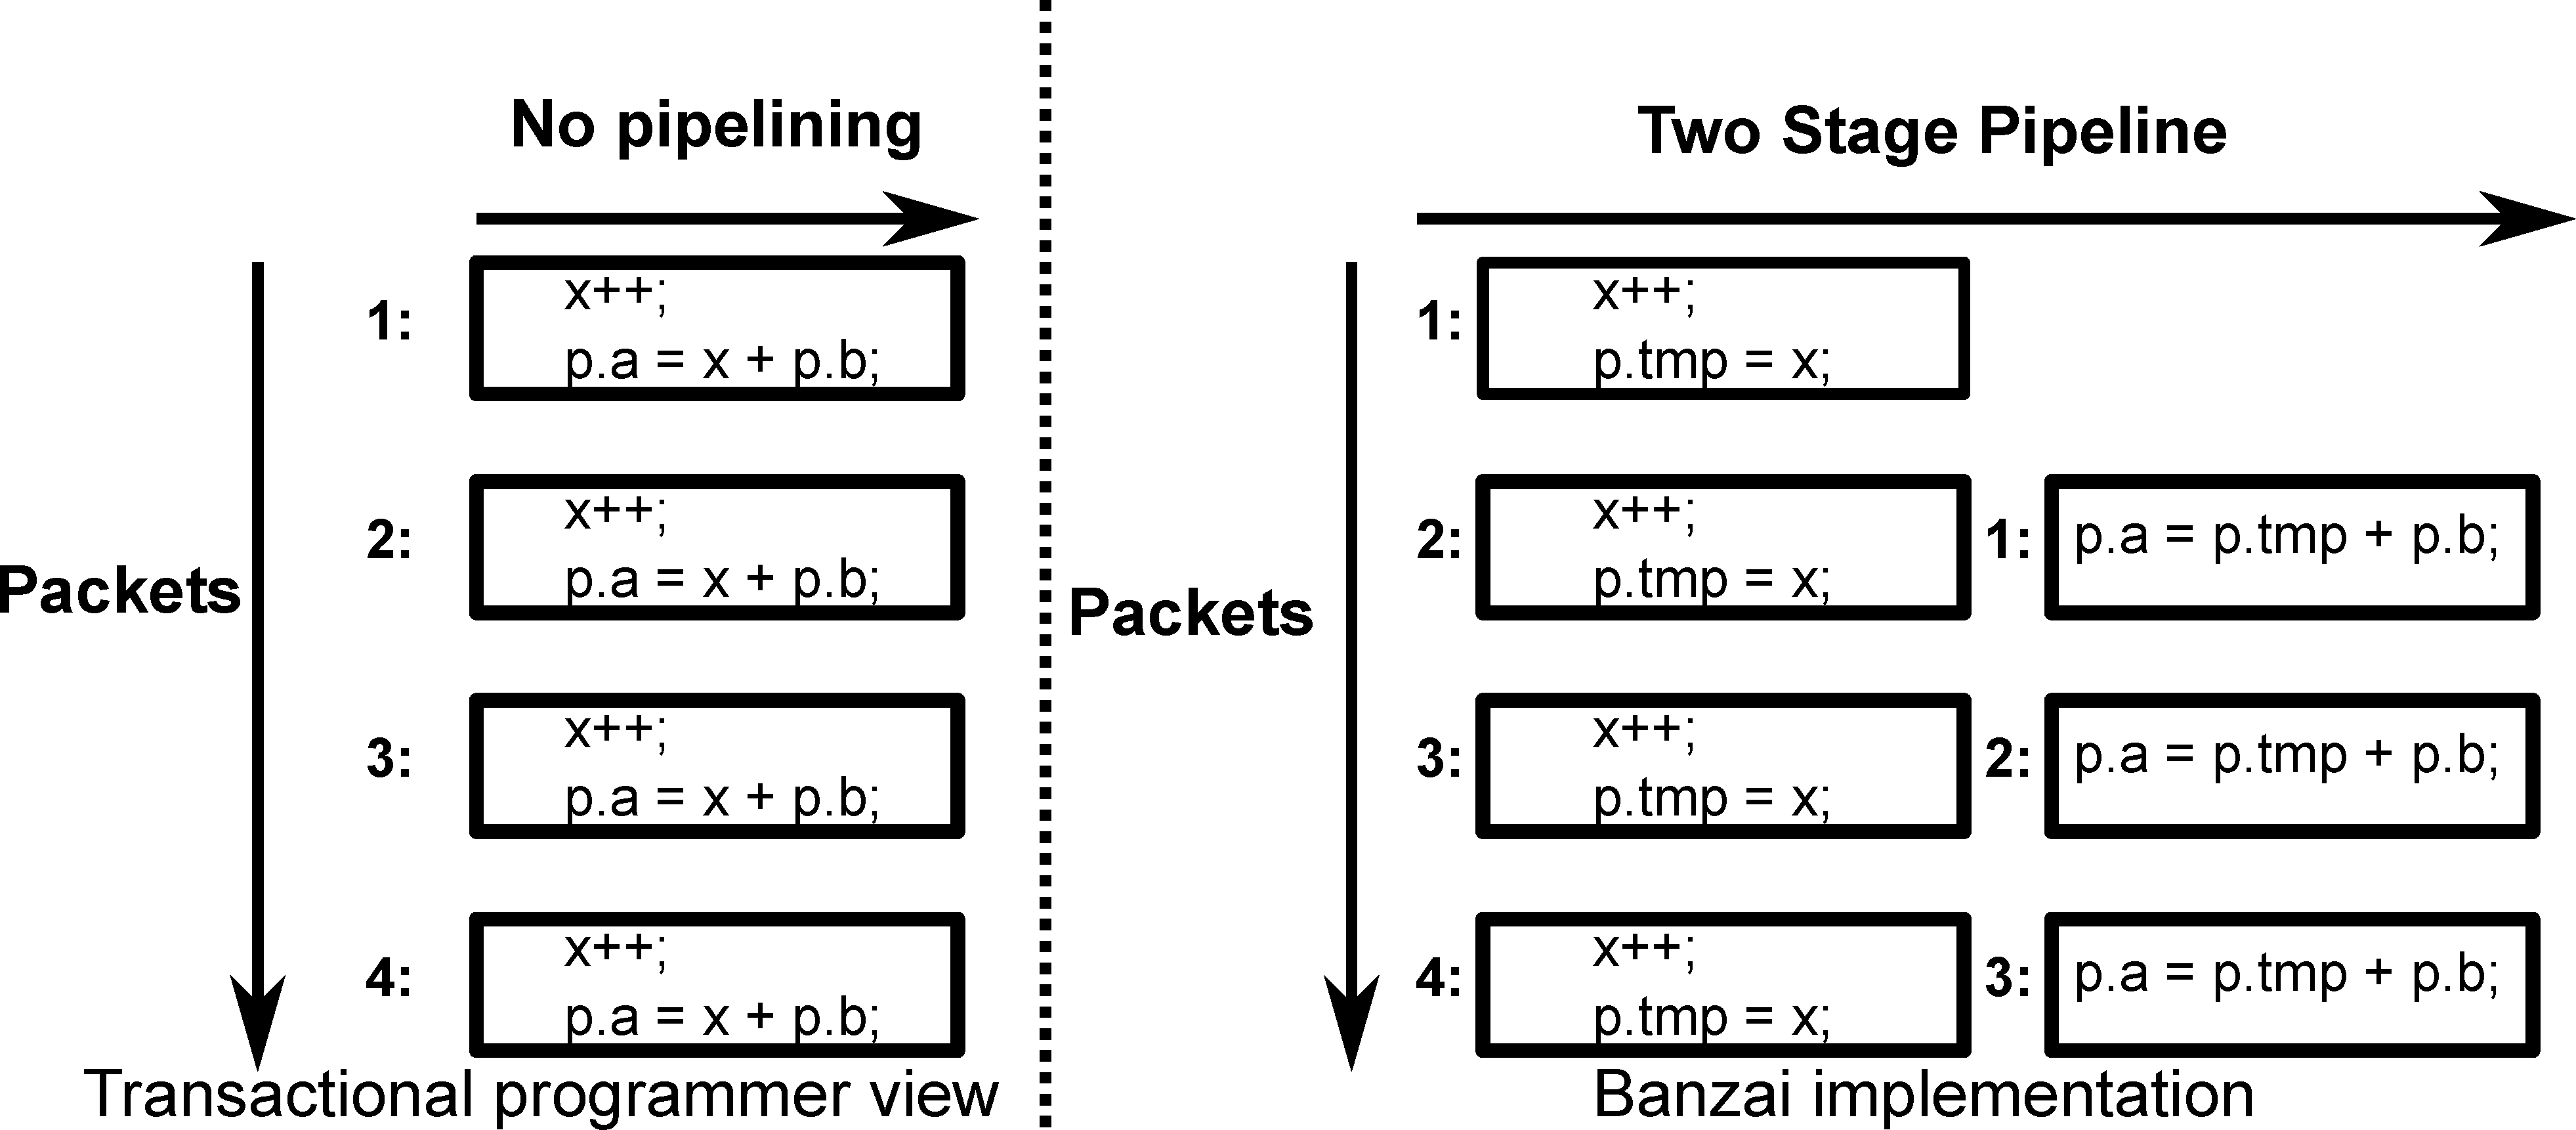
\includegraphics[width=\columnwidth]{spec_vs_impl.pdf}
  \caption{A packet transaction and its implementation}
  \label{fig:trans}
\end{figure}

Transactions are the strongest guarantee that a database system can provide in
that the effect of a transaction is either entirely visible or not with no
intermediate state being visible to the outside world.

We repurpose database transactions for data-plane programming by defining the
notion of a \textit{packet transaction}: a body of sequential code that
executes from start to finish on each packet and conceptually processes only
one packet at a time. For a programmer, the packet transaction represents what
happens to every packet without having to worry about other packets that are
currently being processed or how to parallelize her code. Conceptually, every
packet is processed in isolation and to completion using a sequential block of
code before the next packet's processing begins.

In practice though, switch hardware is heavily pipelined
(Figure~\ref{fig:switch}).  A compiler automatically translates the
programmer's transactional code block into a low-level pipelined implementation
on the switch hardware (Figure~\ref{fig:trans}).

Put differently, the user's packet transaction is a single atom that captures
all computations on the packet and encapsulates all the state required to carry
out the computation.  A compiler then translates this packet transaction into
into a grid of atoms that is functionally equivalent to the single atom, while
respecting hardware constraints on each atom's complexity. If the compiler is
unable to find a mapping, it rejects the packet transaction as being too
complex for the given target.

% TODO: Add a flowlet switching example as a running example here.
